\chapter{The Models Manager}

The model manager tab in the GUI provides the functionality to create models of various types, configure them, specify the variables to use in them, and then estimate their parameters if they have a form that needs to be estimated -- such as regression models or discrete choice models.  A more thorough description of the types of models that can be implemented in OPUS is provided in Chapter \ref{chap:creating-models}.

\begin{figure}[htp]
\begin{center}
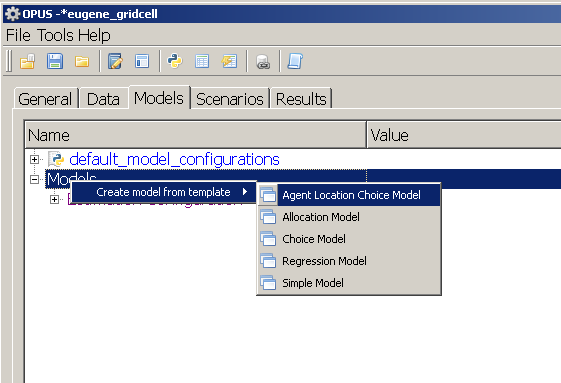
\includegraphics[scale=0.6]{part-gui/images/model-manager-create-model-from-template.png}
\end{center}
\caption{Creating a New Model from a Template}
\label{fig:create-model}
\end{figure}

\section{Creating an Allocation Model}

To demonstrate the process of creating models in the GUI, let's begin with a simple allocation model, which does not have any parameters to estimate and represents a straightforward model to configure.  Say we want to create a model that allocates home-based jobs to zones, and lack sufficient data to specify a choice model or regression model for this purpose.  Home-based jobs are those jobs that are located in properties that are residential in character.  Assume that we have no behavioral information about this problem, other than the insight that home-based jobs are... home-based.  So we can infer that we should probably allocate these jobs to places that have housing (or households).  In allocating these jobs to zones (traffic analysis zones used in the travel model), we can count how many residential units are in each zone, and use this as the weight to allocate the total home-based jobs to zones.  That is, we want to proportionately allocate home-based jobs to zones, weighted by the number of residential units in the zone.  This is equivalent to saying that we want each residential unit to have an equal probability of receiving a home-based job (assuming that we do not have any information to suggest which residential units would be more likely than others to receive such a job).

The next consideration is the capacity of zones to absorb home-based jobs.  One simplifying assumption we could make is that there is a maximum of one home-based job per residential unit in a zone.  On average, our aggregate information suggests that most residential units do not have a home-based job, so this assumtion should not be constraining.

We now have all the information we need to specify a model for home-based jobs.  We will name the model allocate\_home\_based\_jobs, to be descriptive.  The table below contains the \emph{arguments} we will need to use in creating this model in the GUI.

\begin{table}[htp]
\caption{Creating an Allocate Home Based Jobs Model}
\label{tab:allocation-model}
\begin{center}
\begin{tabular}{ p{1.5in}  p{4.4in}  }
\toprule[1.5pt]
Configuration Entry & Value \\
\midrule
Model Name & allocate\_home\_based\_jobs\_model \\
Dataset & zone \\
Outcome Attribute & home\_based\_jobs \\
Weight Attribute & zone.aggregate(building.residential\_units) \\
Control Totals & annual\_employment\_control\_totals \\
Year Attribute & year \\
Capacity Attribute & zone.aggregate(building.residential\_units) \\
\bottomrule
\end{tabular}
\end{center}
\end{table}

The create new model dialog box (Figure {fig:create-model}) contains several kinds of model templates we could create a model from. One of these is Allocation Model. The capacity to create new allocation models, such as this, is now available in the Opus GUI. Select Allocation Model from the list, and a new dialog box appears, with several fields to fill in.  Fill in the fields with the contents from Table \ref{tab:allocation-model}, and save it.  Once this is done, it will appear in the list of models under the Models section of the Model Manager tab.  It is now a fully enabled model, and can be included in a simulation run.

It should go without saying (but doesn't), that creating models through the GUI, with a few mouse clicks and filling in a few fields in a dialog box, is much, much easier than it has been in the past. One does not need to be an expert software developer in order to create and use interesting and fully functional models in OPUS.


\begin{figure}[htp]
\begin{center}
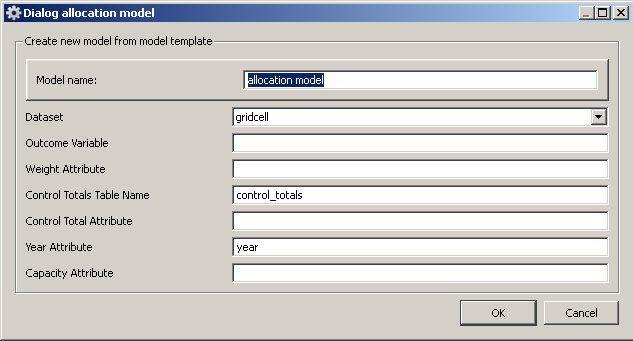
\includegraphics[scale=0.6]{part-gui/images/model-manager-create-allocation-model-from-template.png}
\end{center}
\caption{Creating a New Allocation Model from a Template}
\label{fig:create-allocation-model}
\end{figure}

\section{Creating a Regression Model}

Regression models are also simple to create and specify in the Opus GUI, and can be estimated and simulated within the graphical interface.  We will use as an example the development of a model to predict land values per square foot for all parcels.  Assume we want to create a model that predicts the value of land, per square foot, using the tax assessor valuations of land value and the square footage measures of each parcel available in the assessor data.  Since the outcome is continuous, but truncated at zero and increasing to quite large values, we might want to use a log-transformation of the price per square foot.  This would allow for representing the diminishing returns to larger quantities on some attributes.  We begin, however, with a simple nominal value per square foot, which implies that a unit increase in the amount of an independent variable, adds a constant dollar amount to the value of land per square foot.

The table below summarizes the arguments we would set for creating this model:

\begin{table}[htp]
\caption{Creating a Land Price per Square Foot Model}
\label{tab:land-price-sqft-model}
\begin{center}
\begin{tabular}{ p{1.3in} p{3.0in}  }
\toprule[1.5pt]
Configuration Entry  & Value \\
\midrule
Model Name & land\_price\_model \\
Dataset & gridcell \\
Dependent Variable  &ln\_land\_value   \\
\bottomrule
\end{tabular}
\end{center}
\end{table}

To create this model in the Opus GUI, right-click again on Models, and select in this case Regression Model to generate a new dialog box for this model template, as shown in Figure \ref{fig:create-regression-model}.

\begin{figure}[htp]
\begin{center}
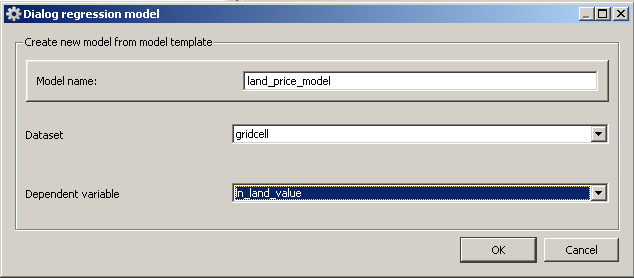
\includegraphics[scale=0.6]{part-gui/images/model-manager-create-regression-model-from-template.png}
\end{center}
\caption{Creating a New Regression Model from a Template}
\label{fig:create-regression-model}
\end{figure}

Once the correct values have been assigned to the configuration of the new model, and you click OK on the dialog box, the model is added to the list of models under Models.  If you expand this node by clicking on the plus sign to the left of the new land price model entry, you will see that it contains a specification and a structure node.  Expand the specification node, and you will find some additional detail, including a reference to submodels, and a variables entry.  We will ignore submodels for now -- it is a means of specifying that you would like to specify the model differently for different subsets of the data.  For now we will just apply a single specification to all the data, to keep this a bit simpler.  We can now move to the task of specifying and estimating this model. 

Right-click on the variables node, and click on Select Variables, as shown in Figure \ref{fig:specify-regression-1}.  At this point a window should appear as shown in Figure \ref{fig:specify-regression-2} that is essentially the same as the variables library window you encountered earlier.  There is a column of check-boxes at the left hand side of the window which you can use to identify the variables you want to include as independent variables, or predictive variables, for this model.  The button at the bottom allows you to accept the selection, which then updates the list of variables in the model specification.  Try adding a constant term, since this is a regression and we need an intercept, or a base value.  Also add a variable like population density.  Now accept the selections.


\begin{figure}[htp]
\begin{center}
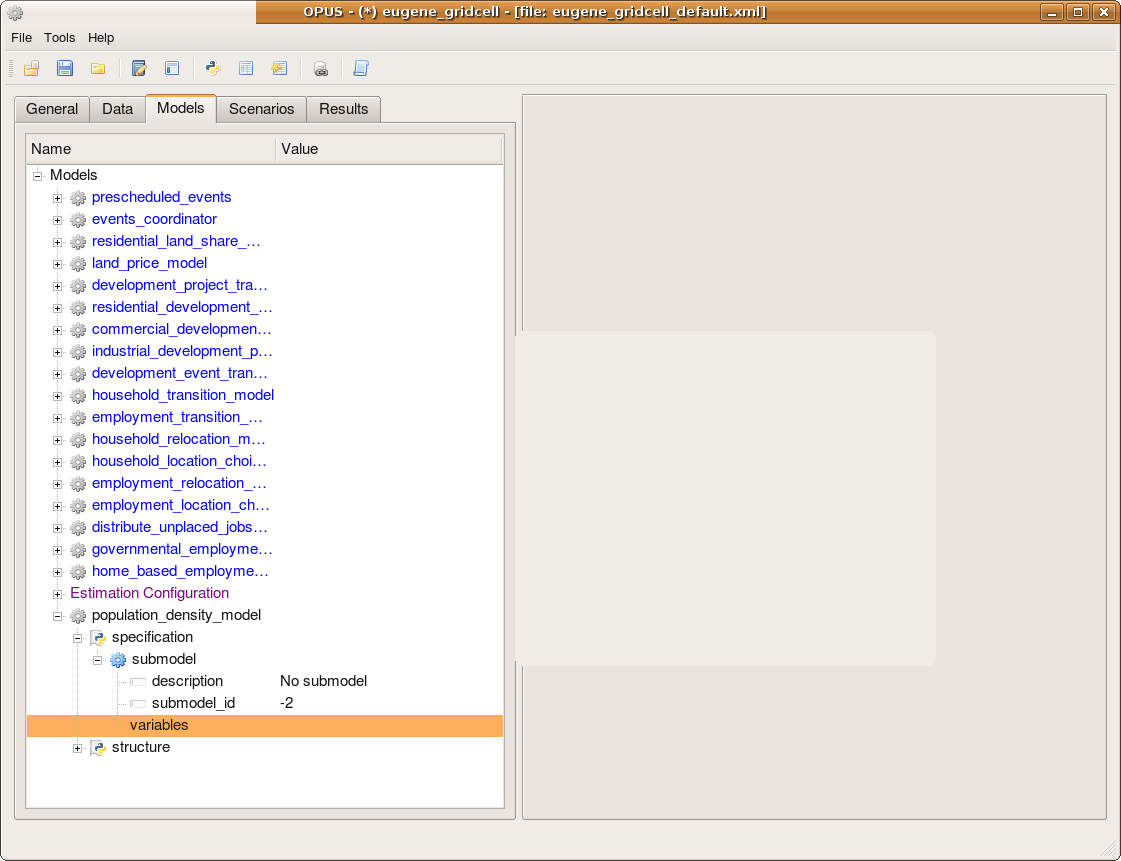
\includegraphics[scale=0.6]{part-gui/images/model-manager-specify-regression-model-1.png}
\end{center}
\caption{Specify the New Land Price Model}
\label{fig:specify-regression-1}
\end{figure}

\begin{figure}[htp]
\begin{center}
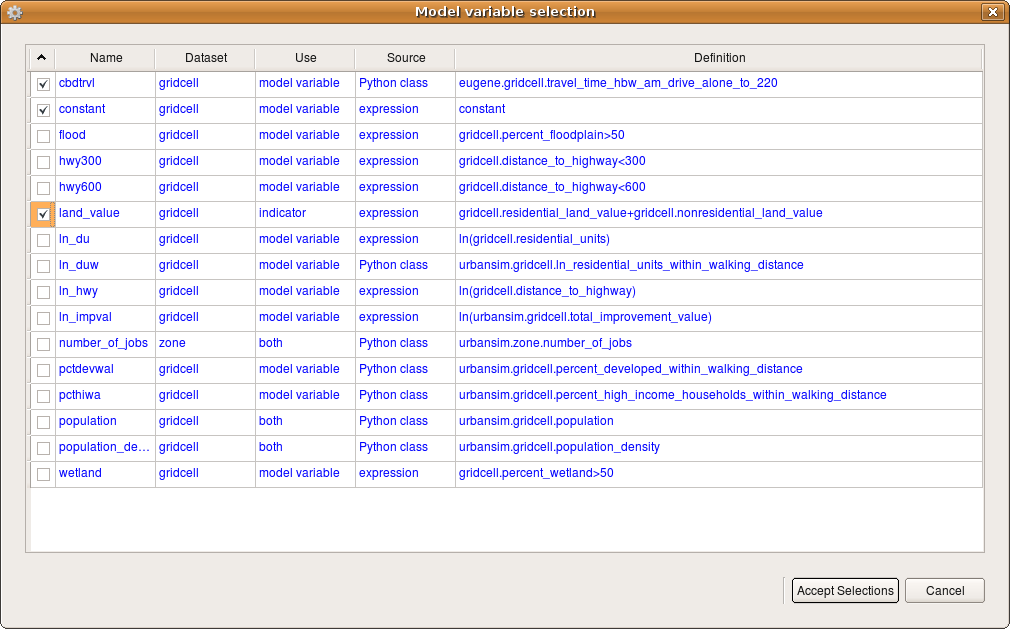
\includegraphics[scale=0.6]{part-gui/images/model-manager-specify-regression-model-2.png}
\end{center}
\caption{Select Variables for Specification}
\label{fig:specify-regression-2}
\end{figure}


Once the model specification has been entered, we can estimate the model parameters using Ordinary Least Squares by right-clicking on the land price model and selecting Run Estimation, as shown in Figure \ref{fig:specify-regression-3}. Once this has been clicked, a new tab appears on the right hand side of the main window, to interact with the model estimation.  Click on the start estimation button, and within a few seconds you should see the estimation results appear in this tab, as shown in Figure \ref{fig:specify-regression-4}.

\begin{figure}[htp]
\begin{center}
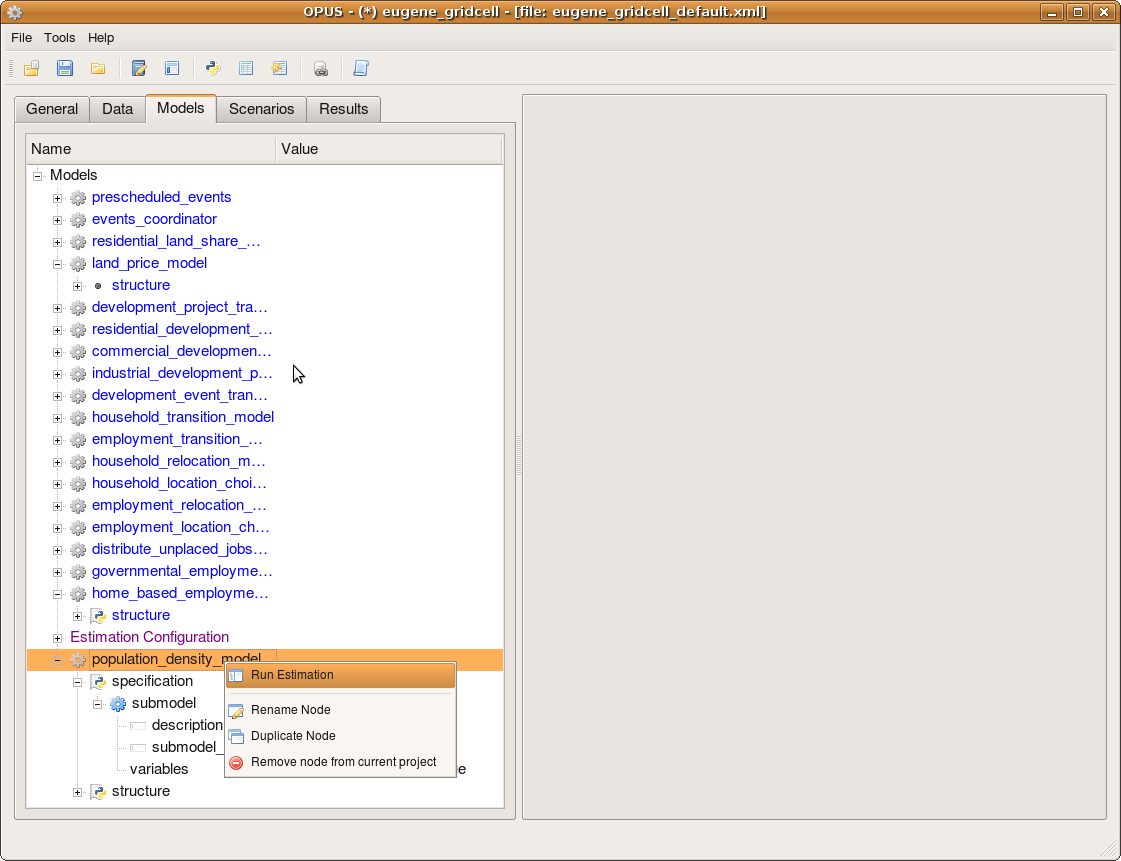
\includegraphics[scale=0.6]{part-gui/images/model-manager-specify-regression-model-3.png}
\end{center}
\caption{Estimate the New Land Price Model}
\label{fig:specify-regression-3}
\end{figure}

\begin{figure}[htp]
\begin{center}
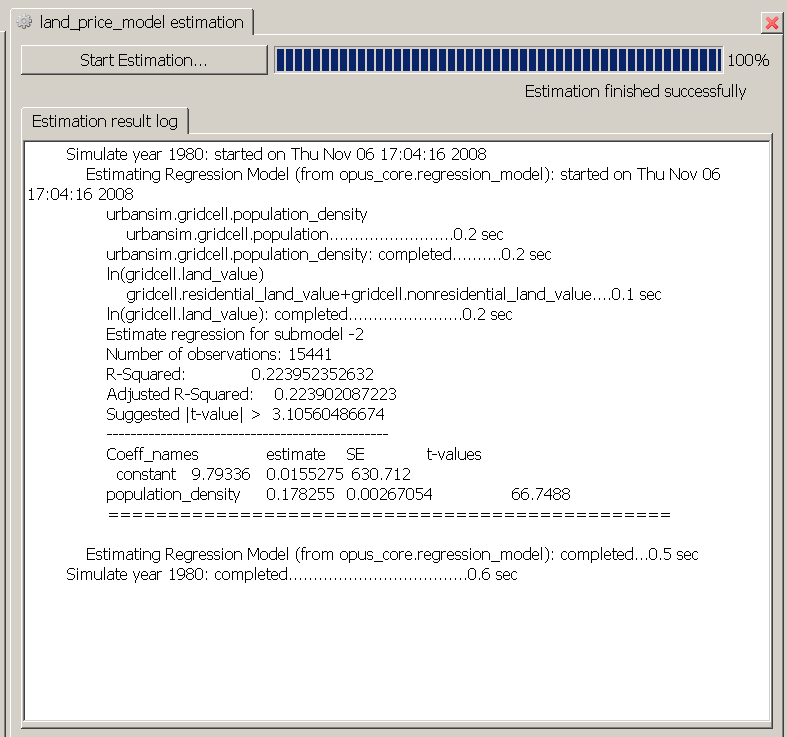
\includegraphics[scale=0.6]{part-gui/images/model-manager-specify-regression-model-4.png}
\end{center}
\caption{Estimation Results}
\label{fig:specify-regression-4}
\end{figure}

We can see from the results that the constant and population density were both quite statistically significant, and that they explain around 22 percent of the variation in land prices in Eugene.  Clearly this is a toy model, but adding other variables in this way can increase the explanatory power to a quite useful level, and as you can see modifying the specification and estimating the model is not difficult to do.

One other note at this point is that the specification and estimation results are automatically stored, if you request this, as shown in Figure  \ref{fig:save-estimation}.  Once the estimation is done, then, the model is ready to use in a simulation, or predictive mode.  More on this in the Scenario Manager section.

\begin{figure}[htp]
\begin{center}
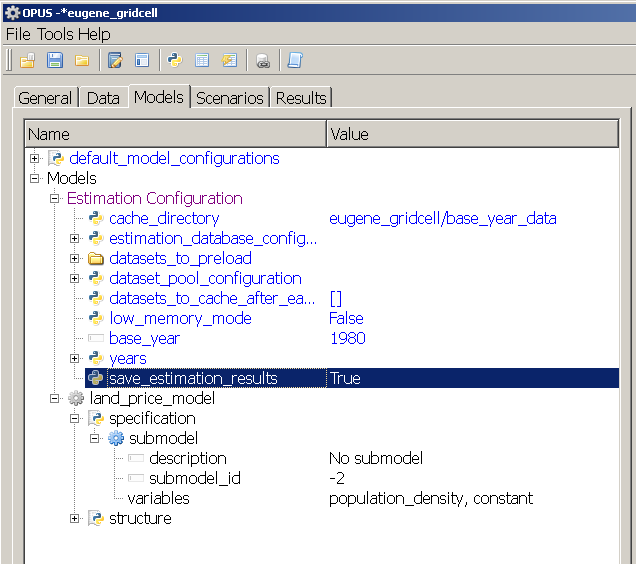
\includegraphics[scale=0.6]{part-gui/images/model-manager-save-estimation.png}
\end{center}
\caption{Save Estimation Results Flag}
\label{fig:save-estimation}
\end{figure}


\section{Creating a Choice Model}
The next type of model we will create is a choice model.  This is a very common modeling application, and is used widely.  Our example for this demonstration is a model of housing type choice, which for purposes of keeping the example simple, we reduce to two alternatives: single-family housing type, or other.  It is likely that households choosing to live in single-family housing may make different trade-offs in other choices, such as travel, and car ownership.  By reducing the model to two outcomes, we create a binary choice model specification.  We always need to use one alternative as a base of comparison in choice models, so for this model we will use the other housing type as the base of comparison.  

Below are the configuration settings for creating a choice model of housing type.  In order to create this model for estimation purposes, we will exclude the few households that are in non-residential property types, and only keep those in multi-family, condominium, and single-family housing.  These are reflected by building type id values of 4, 12, and 19, respectively, in the seattle parcel data.  Filtering the data to include only these three values can be done with the numpy logical\_or command, but since it takes only two arguments, we need to create a nested comparison, as shown below.  Since there are three housing types represented in this data, and we want to create a binary choice outcome for simplicity, it is necessary to create a dependent variable that is 2 if the household occupies a single family house, and 1 otherwise.  In this example, since we will use the entire household table, we draw a small sample of 5\% of the agents to use in estimating the model.

\begin{table}[htp]
\caption{Creating a Housing Type Choice Model}
\label{tab:housing-type-choice-model}
\begin{center}
\begin{tabular}{ p{1.2in}  p{1.2in} p{3.2in}  }
\toprule[1.5pt]
Configuration Entry & Node & Value \\
\midrule
Model Name & & housing\_type\_choice\_model \\
Choice Set & Init & [1, 2] \\
Choice Attribute & Init & single\_family=(household.disaggregate\\ & & (building.building\_type\_id)==19)+1 \\
Estimation Size Agents & Init.Estimation Config & 0.05 \\
Agent Set & Run, Prepare for Run, Estimate, Prepare for Estimate & household \\
Agent Filter & Prepare for Run & numpy.logical\_or(numpy.logical\_or(household.\\ & & disaggregate(building.building\_type\_id)==4,household. \\ & & disaggregate(building.building\_type\_id)==12),household.\\ & & disaggregate(building.building\_type\_id)==19) \\
Specification Table & Prepare for Run & housing\_type\_choice\_model\_specifications \\
Coefficients Table & Prepare for Run, Prepare for Estimate & housing\_type\_choice\_model\_coefficients \\
\bottomrule
\end{tabular}
\end{center}
\end{table}

Figure \ref{fig:configure-choice-model} shows the housing type choice model configuration in progress.  For a binary choice model such as this, the specification of the model is quite similar to the specification of the regression model, but there are some subtle differences.  The most important one is that, as this model is implemented in Opus now, it requires at least one variable in each equation - that is - per alternative.  We typically assign the constant to alternative 1, and all other variables to alternative 2.  In a future revision of the code, the base alternative will not take any variables (this is the more standard implementation).  Figure \ref{fig:choice-model-specification} shows the initial specification of the housing type choice model, with a constant for the other housing types, and income and has\_children included in the utility specification for the single family housing alternative. 

Once the model is specified, it needs to be added to the list of models to estimate, and selected as the model to estimate, as was the case in the preceding regression model example.  Once the model has been added and the project saved, the model can be estimated with the normal right-click option on the models to estimate node.  The results are shown in Figure \ref{fig:choice-model-estimation}.

\begin{figure}[htp]
\begin{center}
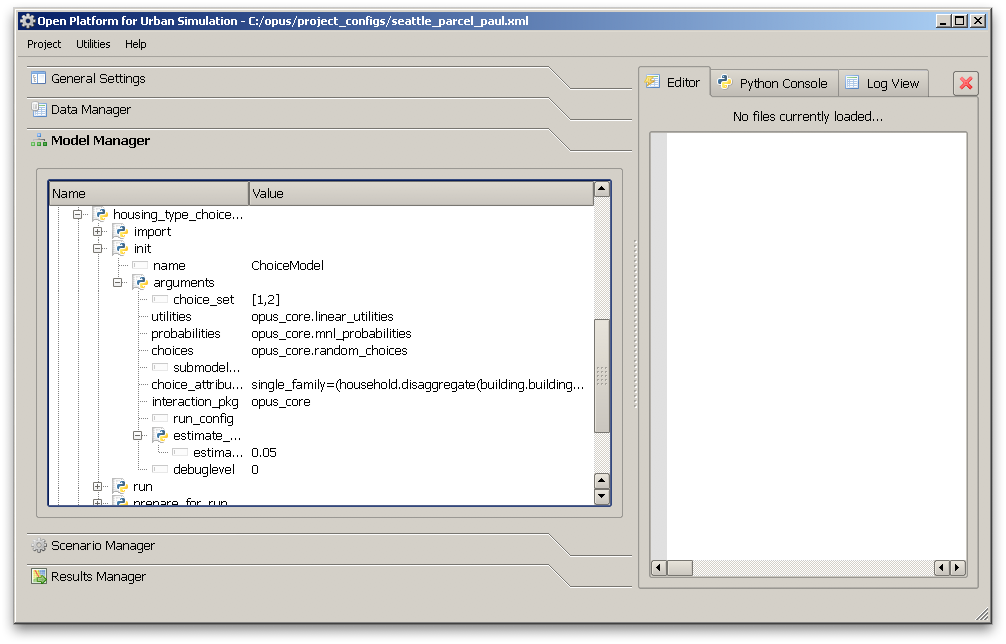
\includegraphics[scale=0.35]{graphics/configure-choice-model.png}
\end{center}
\caption{Configuring the Housing Type Choice Model}
\label{fig:configure-choice-model}
\end{figure}

\begin{figure}[htp]
\begin{center}
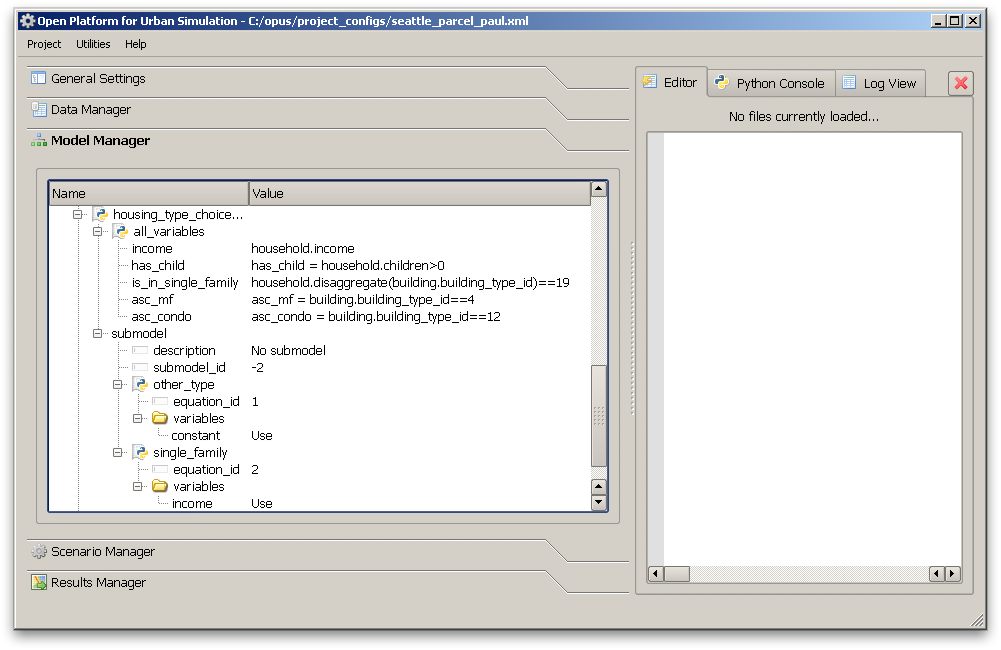
\includegraphics[scale=0.35]{graphics/choice-model-specification.png}
\end{center}
\caption{Specifying the Housing Type Choice Model}
\label{fig:choice-model-specification}
\end{figure}

\begin{figure}[htp]
\begin{center}
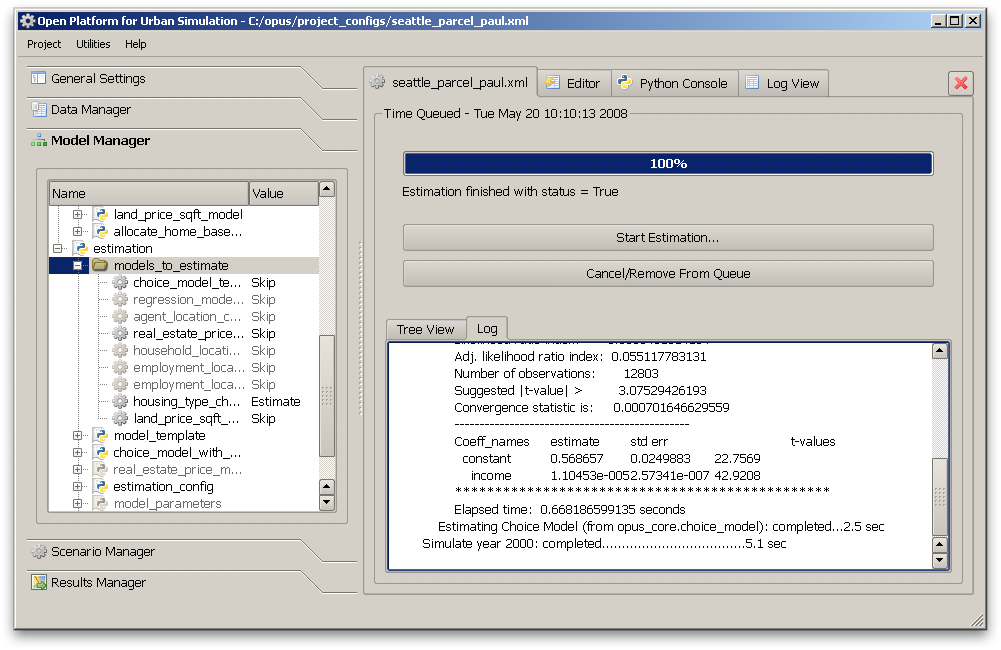
\includegraphics[scale=0.35]{graphics/choice-model-estimation.png}
\end{center}
\caption{Estimating the Housing Type Choice Model}
\label{fig:choice-model-estimation}
\end{figure}
